\chapter{Buoyancy}

When you put a boat into water, it will sink into the water until
the mass of the water it displaces is equal to the mass of the
boat. We think of this in terms of forces. Gravity pulls the mass of
the boat down. The \newterm{buoyant force} pushes the boat up. A boat
dropped into the water will bob up and down a bit before reaching an
equilibrium where the two forces are equal.
% ADD: Explain Action Reaction Pairs in previous chapter
% ADD: Archimedes principle

Watch Khan Academy's introduction to buoyance at \url{https://www.khanacademy.org/science/in-in-class9th-physics-india/in-in-gravity/in-in-pressure-in-liquids-archimedes-principle/v/archimedes-principle-buoyancy-fluids-physics-khan-academy}

The buoyant force pushes things up -- against the force of
gravity. The force is equal to the weight of the fluid being
replaced. So, for example, a cubic meter of freshwater has a mass of
about 1000kg.  If you submerge anything with a volume of one meter in
freshwater on earth, the buoyant force will be about 9800 newtons.

For some things, like a block of styrofoam, this buoyant force will be
sufficient to carry it to the surface. Once it reaches the surface, it
will continue to rise (displacing less water) until the mass of the
water it displaces is equal to its mass. And then we say ``It floats!''

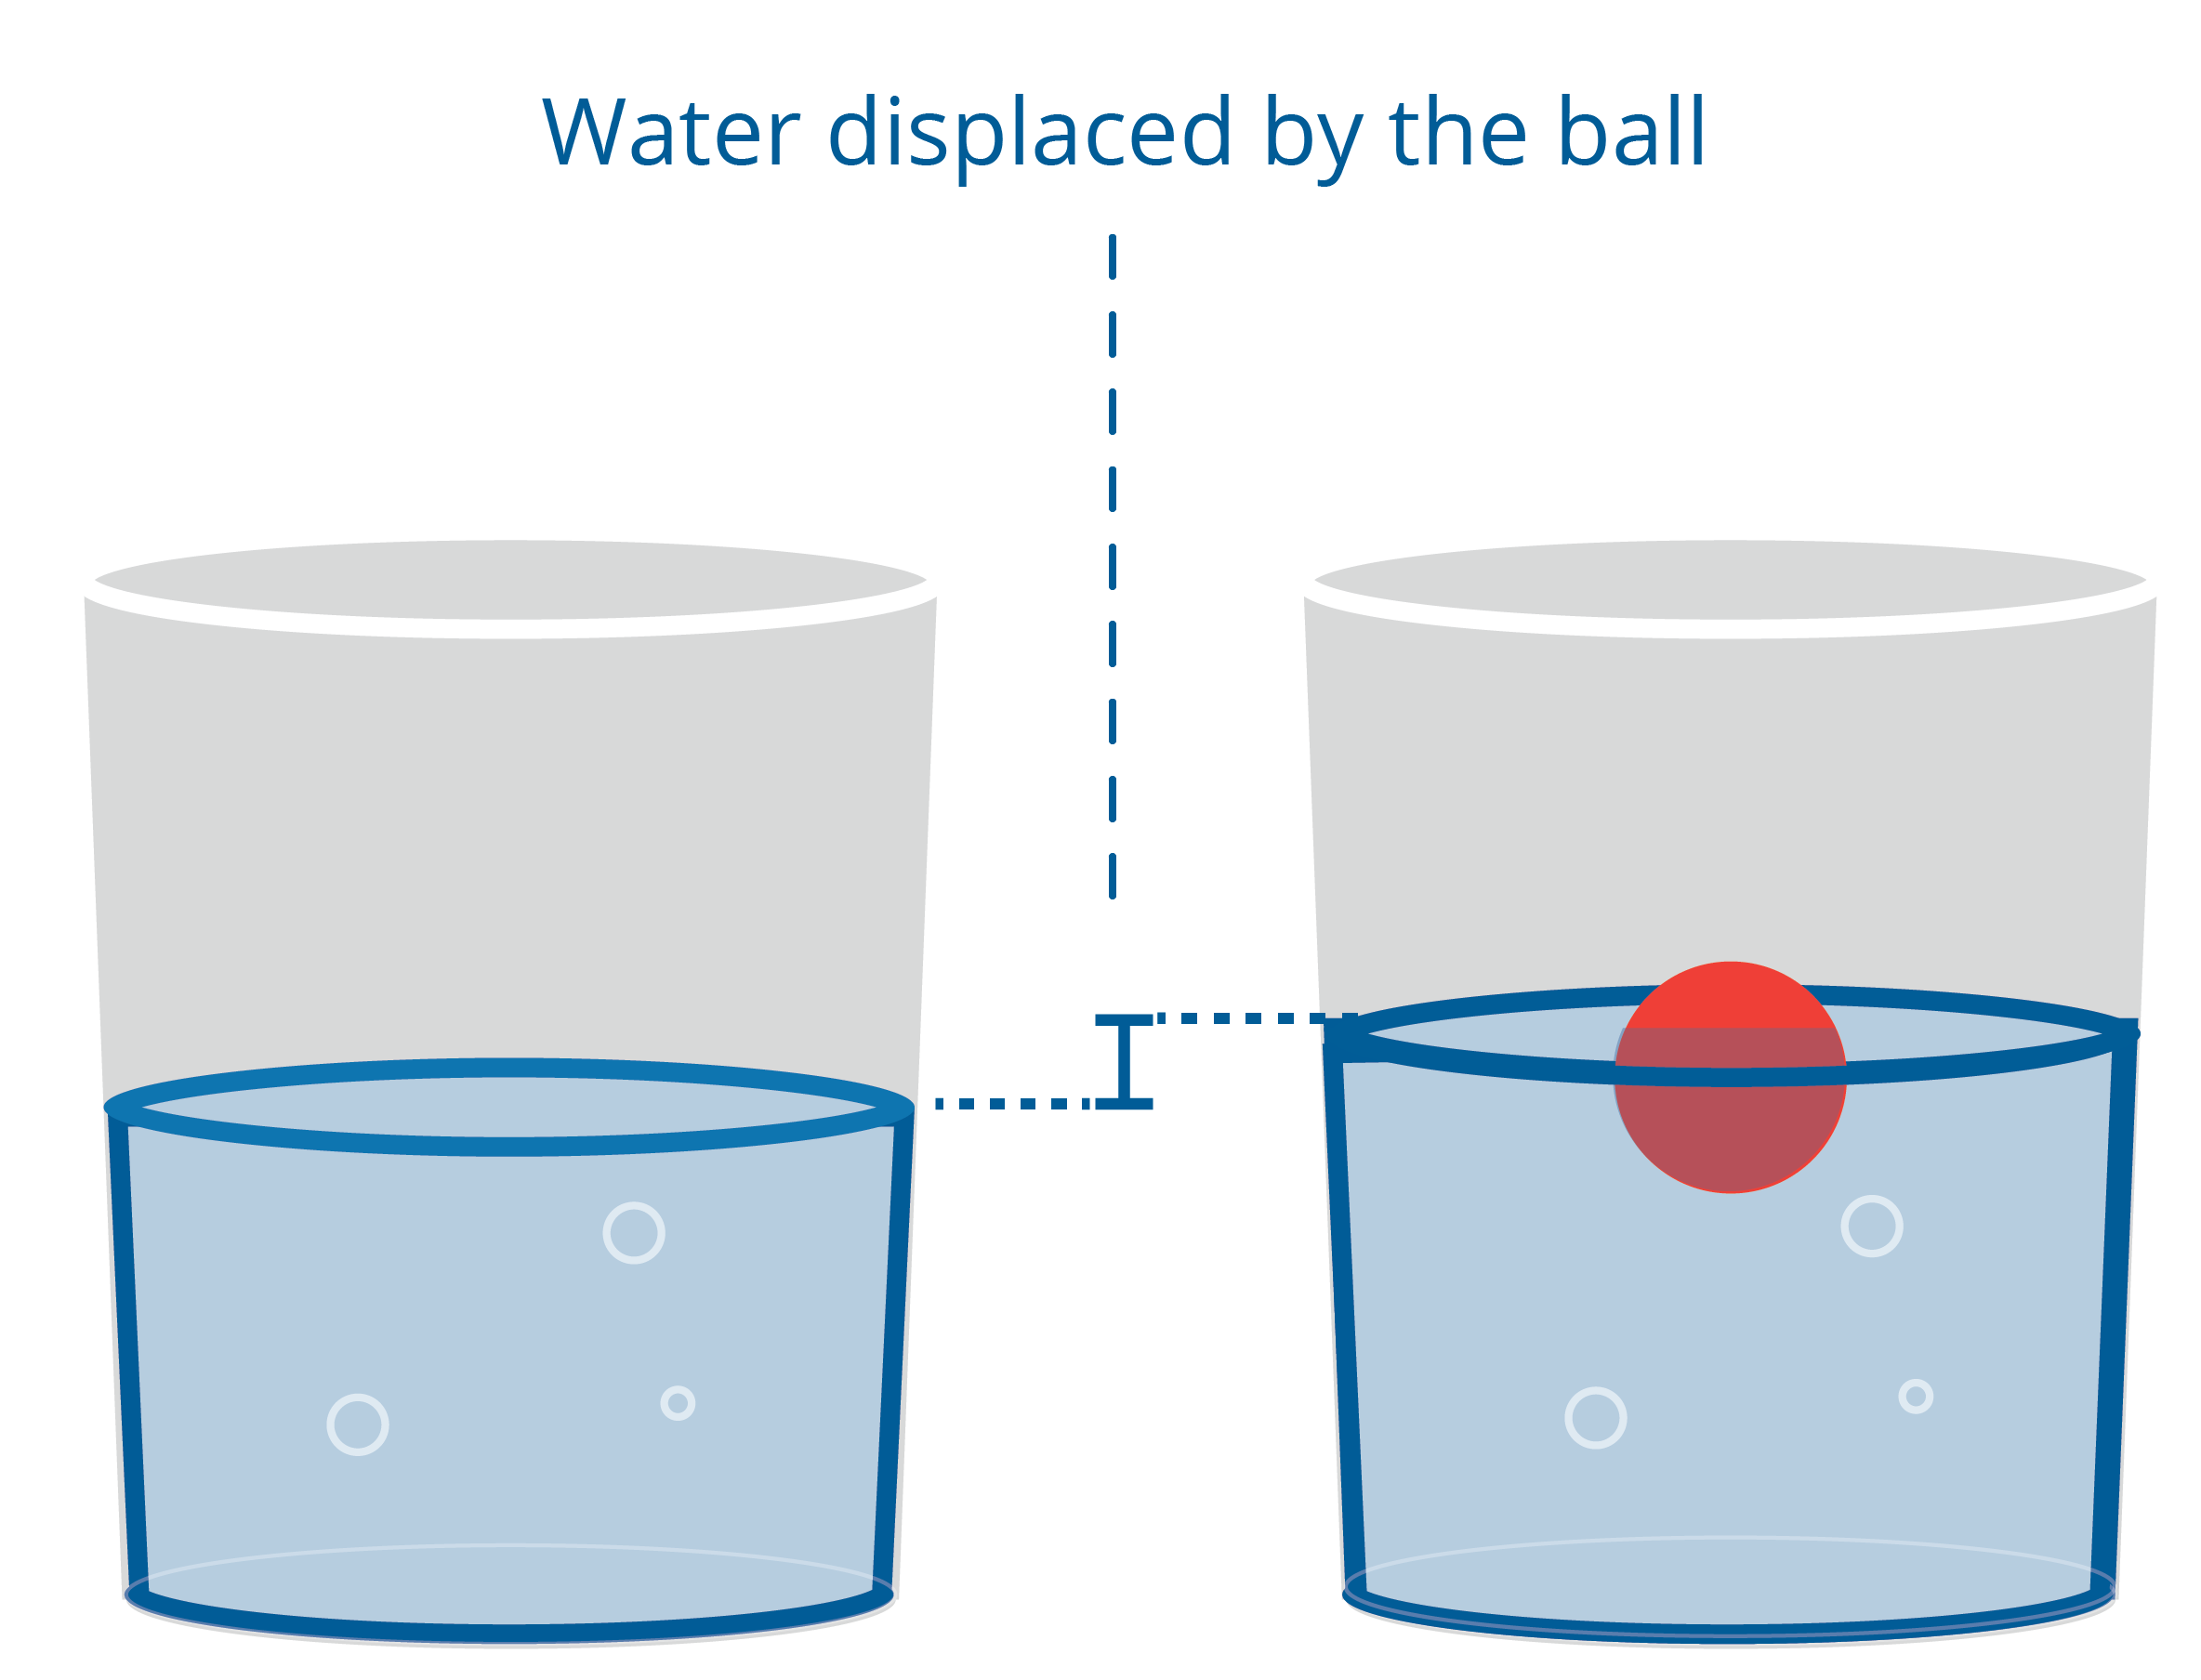
\includegraphics[width=1\textwidth]{waterDisplacement.png}

For some things, like a block of lead, the buoyant force is not
 sufficient to lift it to the surface, and thus we say ``It sinks!''

This is why a helium balloon floats through the air. The air
that it displaces weighs more than the balloon and the helium itself. (It is easy to forget that air has a mass, but it does.)

\begin{Exercise}[title={Buoyancy}, label=buoyancy]
  You have an aluminum box that has a heavy base, so it will always
  float upright. The box and its contents weigh 10 kg. Its base is 0.3 m x 0.4 m. It is 1m tall.

  When you drop it into freshwater ($1000 kg/m^3$), how far will it sink
  before it reaches equilibrium.
  
\end{Exercise}
\begin{Answer}[ref=buoyancy]
  Equilibrium will be achieved when the box has displaced 10 kg of water. That is, when it has displaced $0.01$ cubic meters.

  The area of the base of the box is 0.12 square meters.  So if the
  box sinks $x$ meters into the water it will displace $0.12 x$ cubic
  meters.

  Thus at equilibrium $x = \frac{0.01}{0.12} \approx 0.083$ m.  So,
  the box will sink 8.3 cm into the water before reaching equilibrium.
\end{Answer}

\section{The Mechanism of Buoyancy}

As you dive down in the ocean, you will experience greater and
greater pressure from the water. And if you take a balloon with you, you
will gradually see it get smaller as the water pressure compresses the
air in the balloon.

Let's say you are 3 meters below the surface of the water. What is the
pressure in Pascals (newtons per square meter)? You can think of the
water as a column of water crushing down upon you. The pressure over
a square meter is the weight of 3 cubic meters of water pressing down.

$$p = (3)(1000)(9.8) = 29,400 \text{ Pa }$$

This is called \newterm{hydrostatic pressure}. The general rule for
hydrostatic pressure in Pascals $p$ is

$p = d g h$

Where  $d$ is the density of the fluid
in kg per cubic meter, $g$ is the acceleration due to gravity in
$m/s^2$, and $h$ is the height of the column of fluid above you.

So, where does buoyant force come from? Basically, the pressure pushing up on the
deepest part of the object is higher than the pressure pushing down on
the shallowest part of the object. That is where bouyancy comes from.

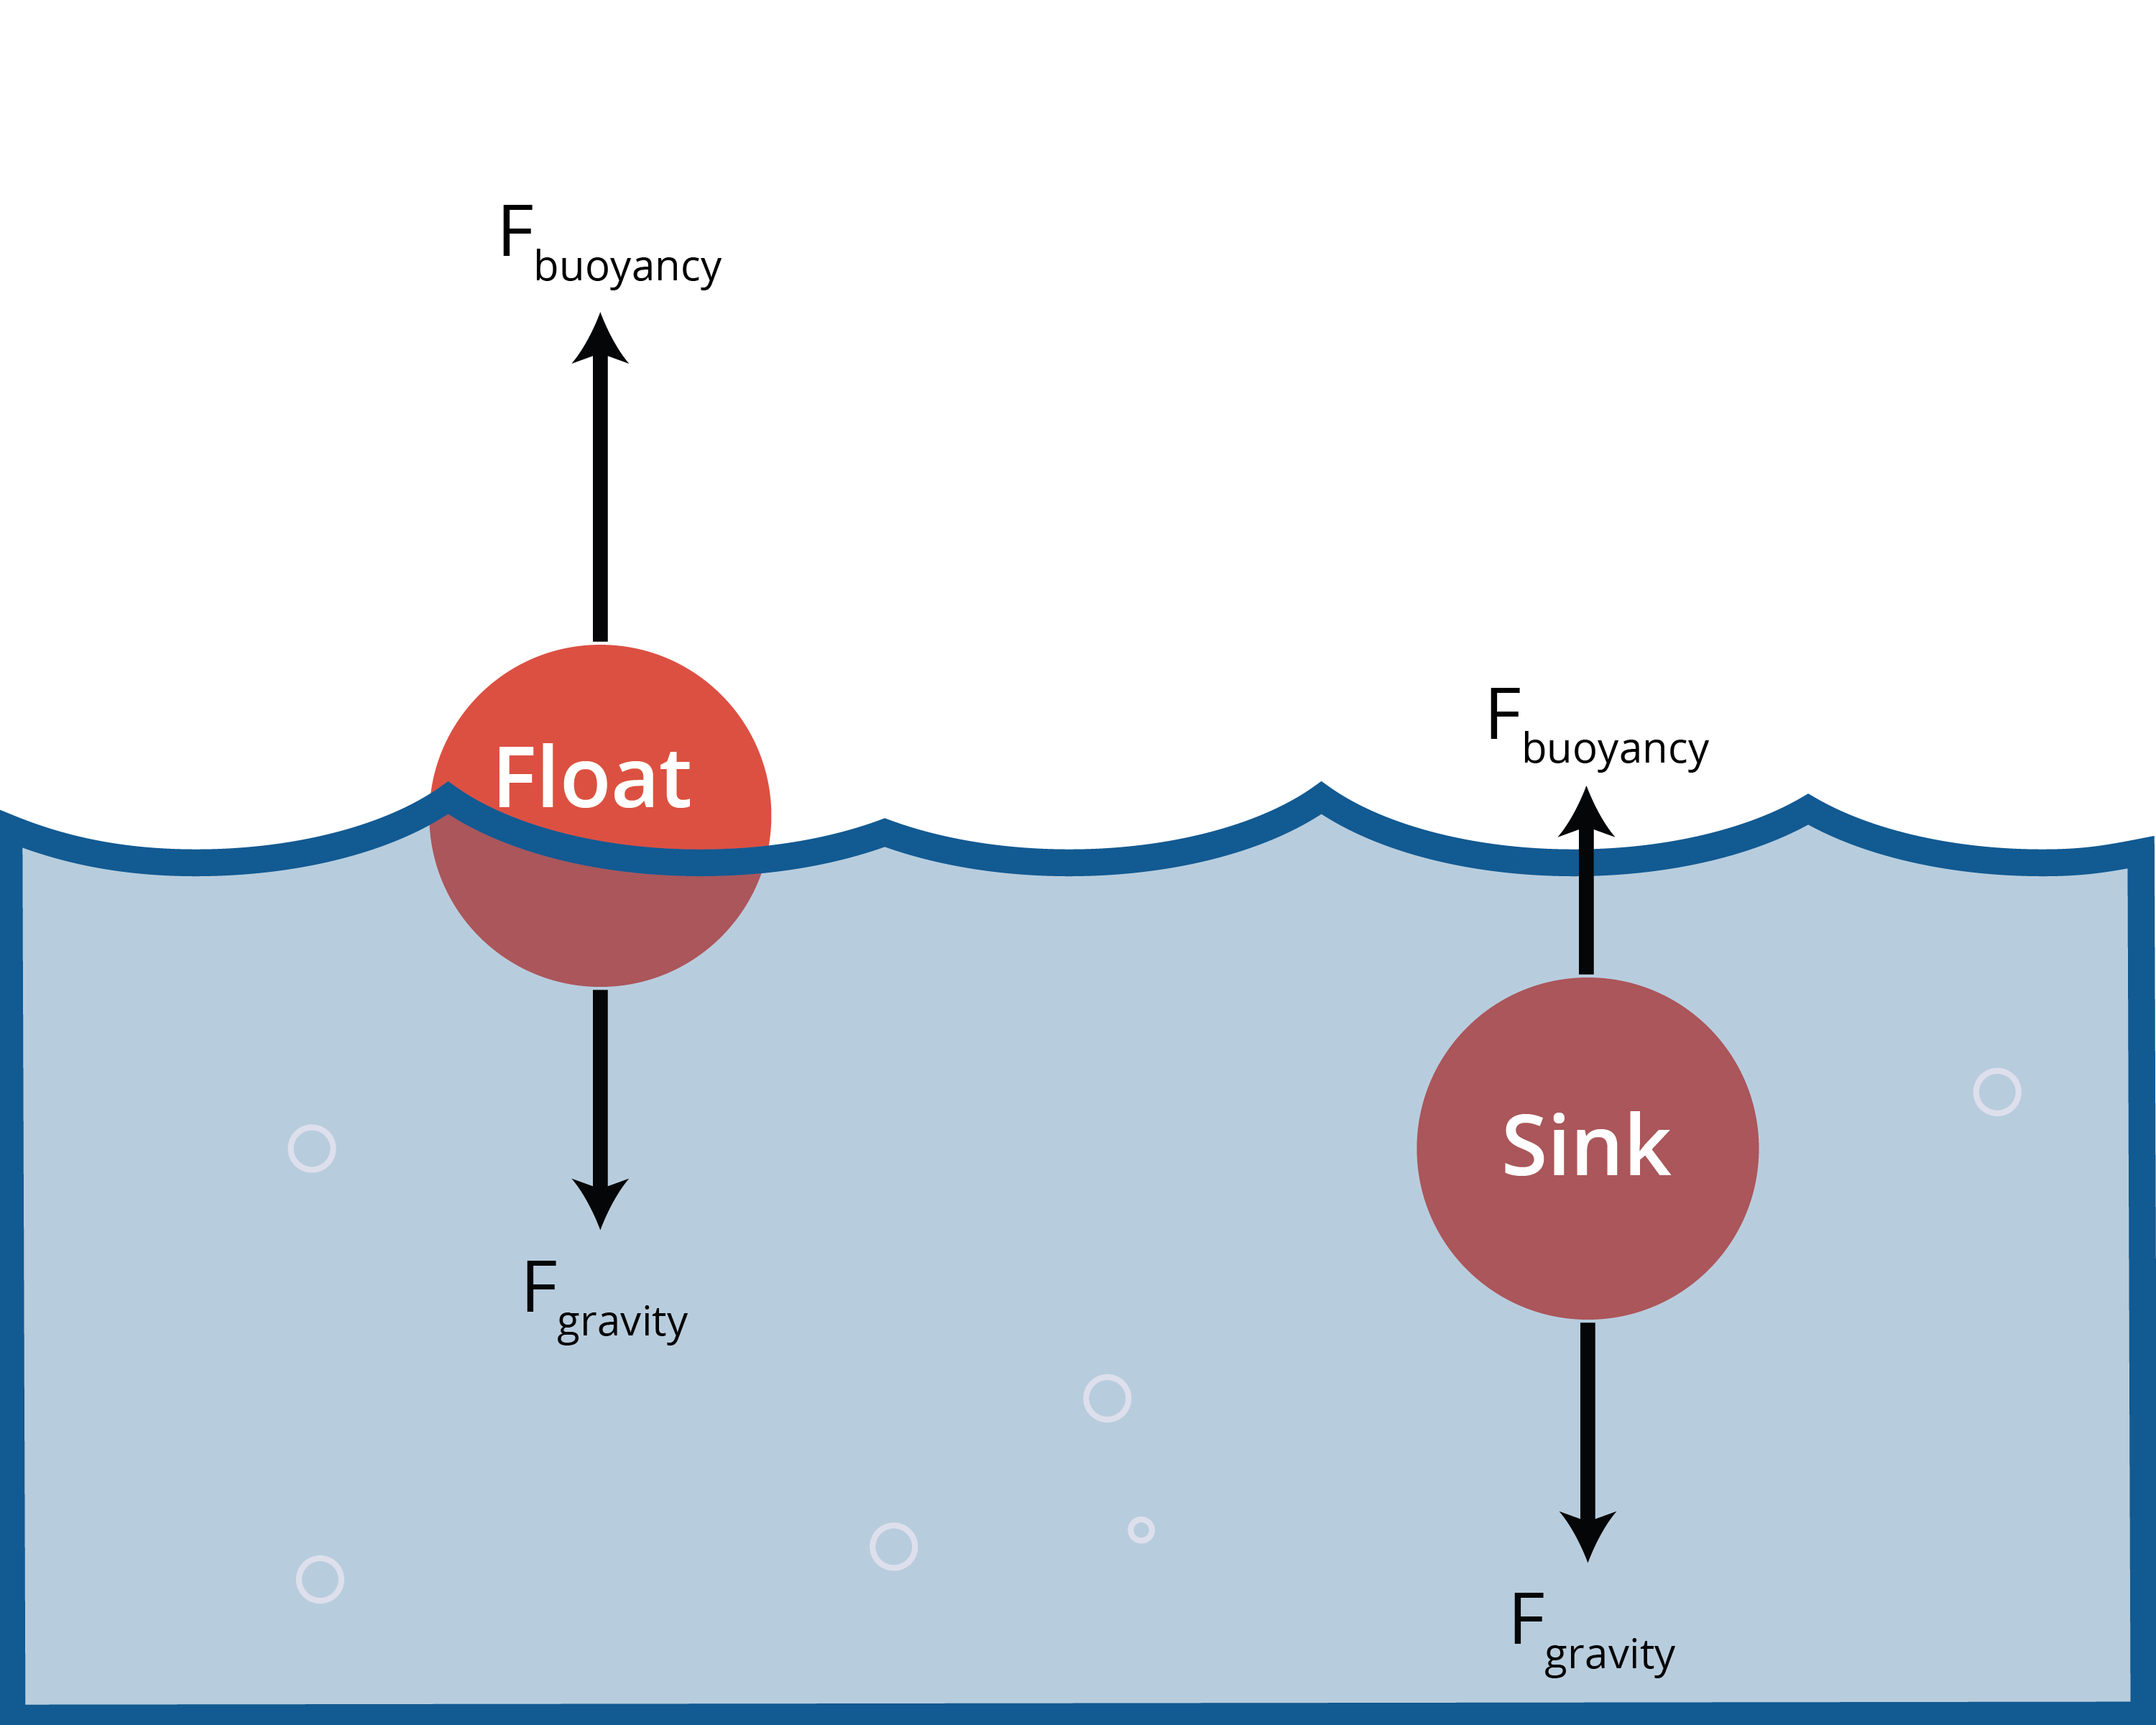
\includegraphics[width=1\textwidth]{buoyancy.png}

\begin{Exercise}[title={Hydrostatic Pressure}, label=mars_pressure]

  You dive into a tank of olive oil on Mars. How much more
  hydrostatic pressure does your body experience at 5 meters deep than
  it did at the surface?

  The density of olive oil is about 900 kg per square meter. The
  acceleration due to gravity on Mars is 3.721 $m/s^2$.
  
\end{Exercise}
\begin{Answer}[ref=mars_pressure]
$$p = d g h = (900)(3.721)(5) = 16,744.5 \text{ Pa}$$
\end{Answer}

Notice that although the pressure is increasing as you go deeper, the
buoyant force will \emph{not increase} because the buoyant force is always equal
to the weight of the fluid that is displaced, regardless if that is 1
meter or 100 meters underwater.

Also, saltwater is denser then freshwater. That is why people float
better in the sea than they do in a river.

And, lipids, like fats and oils, are less dense than water. That is why
people with a lot of body fat tend to float better than people with
less body fat. And why oil floats in a glass of water.

